\documentclass[10pt, oneside]{amsart}
% \usepackage[showboxes]{textpos}

\usepackage[absolute,overlay]{textpos}
	\setlength{\TPHorizModule}{1.0cm}
	\setlength{\TPVertModule}{\TPHorizModule}
	\textblockorigin{0.0cm}{0.0cm}  %start all at upper left corner

\usepackage{amsmath}
\usepackage{amsthm}
\usepackage{amsfonts}
\usepackage{amssymb}
\usepackage{mathpazo}
\usepackage{booktabs}
\usepackage[usenames,x11names]{xcolor}
\usepackage{tikz}
\usepackage{textcomp}
\usepackage[letterpaper]{geometry}
\geometry{verbose,tmargin=0.5in,bmargin=0.5in,lmargin=1in,rmargin=0.5in}
\usepackage{multicol}
\usepackage{bm}
\usepackage{comment}
\usepackage{cancel}
\usepackage{array}
\usepackage{gensymb}
\usepackage{enumerate}

\pagestyle{plain}
\raggedright
\renewcommand{\familydefault}{\sfdefault}
\setlength{\parskip}{\medskipamount}
\setlength{\columnsep}{1cm}

\everymath{\displaystyle}
\setlength{\parskip}{\bigskipamount}
% \setlength{\oddsidemargin}{15.5pt}
% \setlength{\evensidemargin}{15.5pt}

% \input{../macros2013}
\input{../../macros}

\begin{document}

\thispagestyle{empty}
\vspace{-7cm}

\begin{center}
	\textbf{\Large Module 6: Minor Losses (CIVL 318)}
	\par\medskip
\end{center}

\cmini[0.5]{
	\begin{align*}
 	f &= \frac{0.25}{\left[\log\left(\frac{1}{3.7\left(D/\epsilon\right)}+\frac{5.74}{N_R^{0.9}}\right)\right]^2}  \\\\
	h_L &= K\cdot\frac{v^2}{2g}\\
 	\intertext{Flow through valves:}
	h_L &= f_T\cdot \frac{L_e}{D}\cdot \frac{v^2}{2g}
	% \intertext{where}
	% K &= f_T\left(\frac{L_e}{D}\right)
\end{align*}
}
\centering
\par\vspace{1cm}

\textbf{K-values for Sudden Contraction}

\begin{center}
	\begin{tabular}{>{$}c<{$} >{$}c<{$} >{$}c<{$} >{$}c<{$}>{$}c<{$}>{$}c<{$} >{$}c<{$} >{$}c<{$} >{$}c<{$} >{$}c<{$}
		>{$}c<{$} }
	 	\toprule
	 	\addlinespace
	 	 && \multicolumn{9}{c}{Velocity, $v$} \\
	 	D_1/D_2 &\qquad& 0.6\,\text{m/s} & 1.2\,\text{m/s} & 1.8\,\text{m/s} & 2.4\,\text{m/s}& 3\,\text{m/s} &
	 	4.5\,\text{m/s} & 6\,\text{m/s} & 9\,\text{m/s} & 12\,\text{m/s} \\
	 	\midrule 1 && 0.0 & 0.0 & 0.0 & 0.0 & 0.0 & 0.0
	 	& 0.0  & 0.0 & 0.0\\
	 	1.1 && 0.03 & 0.04 & 0.04 & 0.04 & 0.04 & 0.04 & 0.05 & 0.05 & 0.06\\
	 	1.2 && 0.07 & 0.07 & 0.07 & 0.07 & 0.08 & 0.08 & 0.09 & 0.10 & 0.11 \\
	 	1.4 && 0.17 & 0.17 & 0.17 & 0.17 & 0.18 & 0.18 & 0.18 & 0.19 & 0.20 \\
	 	1.6 && 0.26 & 0.26 & 0.26 & 0.26 & 0.26 & 0.25 & 0.25 & 0.25 & 0.24 \\
	 	1.8 && 0.34 & 0.34 & 0.34 & 0.33 & 0.33 & 0.32 & 0.31 & 0.29 & 0.27 \\
	 	2.0 && 0.38 & 0.37 & 0.37 & 0.36 & 0.36 & 0.34 & 0.33 & 0.31 & 0.29 \\
	 	2.2 && 0.40 & 0.40 & 0.39 & 0.39 & 0.38 & 0.37 & 0.35 & 0.33 & 0.30 \\
	 	2.5 && 0.42 & 0.42 & 0.41 & 0.40 & 0.40 & 0.38 & 0.38 & 0.34 & 0.31 \\
	 	3.0 && 0.44 & 0.44 & 0.43 & 0.42 & 0.42 & 0.40 & 0.39 & 0.36 & 0.33 \\
	 	4.0 && 0.47 & 0.46 & 0.45 & 0.45 & 0.44 & 0.42 & 0.41 & 0.37 & 0.34  \\
	 	5.0 && 0.48 & 0.47 & 0.47 & 0.46 & 0.45 & 0.44 & 0.42 & 0.38 & 0.35 \\
	 	10.0 && 0.49 & 0.48 & 0.48 & 0.47 & 0.46 & 0.45 & 0.43 & 0.40 & 0.36 \\
	 	\infty && 0.49 & 0.48 & 0.48 & 0.47 & 0.47 & 0.45 & 0.44 & 0.41 & 0.38 \\
	 	\bottomrule
	\end{tabular}
\end{center}
\par\vspace{1cm}


	\textbf{K-values for Gradual Contraction}

	\begin{equation*}
		K=
		\begin{cases}
			0.5\sqrt{\sin\frac{\theta}{2}}\left(1-\left(\frac{D_2}{D_1}\right)^2\right), & 45\degree < \theta \le 180\degree
			\\
			 0.8\sin\frac{\theta}{2}\left(1-\left(\frac{D_2}{D_1}\right)^2\right), & 15\degree < \theta \le 45\degree
		\end{cases}
	\end{equation*}
	\par
			where $D_2$ is the smaller (downstream) diameter of the pipe after the contraction and $D_1$ is the diameter of the
			larger (upstream) pipe and the head loss is based on the velocity of the smaller pipe.

\par\bigskip
\hrule
%\textbf{K-values for Sudden Enlargement}
%
%For $v\approx 1.2\,\text{m/s},\quad K=\left[1-\left(\frac{D_1}{D_2}\right)^2\right]^2  $
\newpage
\textbf{K-values for Sudden Enlargement}:\par
\begin{center}


\begin{tabular}{>{$}c<{$} >{$}c<{$} >{$}c<{$} >{$}c<{$} >{$}c<{$} >{$}c<{$} >{$}c<{$} >{$}c<{$} >{$}c<{$} }
		 	\toprule
		 	\addlinespace
		 	 && \multicolumn{7}{c}{Velocity, $v$} \\
		 	D_2/D_1 &\qquad& 0.6\,\text{m/s} & 1.2\,\text{m/s} & 3\,\text{m/s} & 4.5\,\text{m/s}  & 6\,\text{m/s}  &
		 	9\,\text{m/s} & 12\,\text{m/s} \\ \midrule
		 	1 && 0.0 & 0.0 & 0.0 & 0.0 & 0.0 & 0.0 & 0.0 \\
		 	1.2 && 0.11 & 0.10 & 0.09 & 0.09 & 0.09 & 0.09 & 0.08 \\
		 	1.4 && 0.26 & 0.25 & 0.23 & 0.22 & 0.22 & 0.21 & 0.20 \\
		 	1.6 && 0.40 & 0.38 & 0.35 & 0.34 & 0.33 & 0.32 & 0.32 \\
		 	1.8 && 0.51 & 0.48 & 0.45 & 0.43 & 0.42 & 0.41 & 0.40 \\
		 	2.0 && 0.60 & 0.56 & 0.52 & 0.51 & 0.50 & 0.48 & 0.47 \\
		 	2.5 && 0.74 & 0.70 & 0.65 & 0.63 & 0.62 & 0.60 & 0.58 \\
		 	3.0 && 0.83 & 0.78 & 0.73 & 0.70 & 0.69 & 0.67 & 0.65 \\
		 	4.0 && 0.92 & 0.87 & 0.80 & 0.78 & 0.76 & 0.74 & 0.72 \\
		 	5.0 && 0.96 & 0.91 & 0.84 & 0.82 & 0.80 & 0.77 & 0.75 \\
		 	10.0 && 1.00 & 0.96 & 0.89 & 0.86 & 0.84 & 0.82 & 0.80 \\
		 	\infty && 1.00 & 0.98 & 0.91 & 0.88 & 0.86 & 0.83 & 0.81 \\
		 	\bottomrule
		\end{tabular}

\end{center}
\par\vspace{1cm}

\textbf{K-values for Gradual Enlargement}

\begin{center}
	\begin{tabular}{>{$}c<{$} >{$}c<{$} >{$}c<{$} >{$}c<{$} >{$}c<{$} >{$}c<{$} >{$}c<{$} >{$}c<{$} >{$}c<{$} >{$}c<{$}
 		>{$}c<{$} >{$}c<{$} >{$}c<{$} }
 		\toprule
 		D_2/D_1 & 2^\circ & 6^\circ & 10^\circ & 15^\circ & 20^\circ & 25^\circ & 30^\circ & 35^\circ & 40^\circ & 45^\circ & 50^\circ & 60^\circ\\
 		\midrule
		1.1 & 0.01 & 0.01 & 0.03 & 0.05 & 0.10 & 0.13 & 0.16 & 0.81 & 0.19 & 0.20 & 0.21 & 0.23 \\

		1.2 & 0.02 & 0.02 & 0.04 & 0.09 & 0.16 & 0.21 & 0.25 & 0.29 & 0.31 & 0.33 & 0.35 & 0.37 \\

		1.4 & 0.02 & 0.03 & 0.06 & 0.12 & 0.23 & 0.30 & 0.36 & 0.41 & 0.44 & 0.47 & 0.50 & 0.53 \\

		1.6 & 0.03 & 0.04 & 0.07 & 0.14 & 0.26 & 0.35 & 0.42 & 0.47 & 0.51 & 0.54 & 0.57 & 0.61 \\

		1.8 & 0.03 & 0.04 & 0.07 & 0.15 & 0.28 & 0.37 & 0.44 & 0.50 & 0.54 & 0.58 & 0.61 & 0.65 \\

		2.0 & 0.03 & 0.04 & 0.07 & 0.16 & 0.29 & 0.38 & 0.46 & 0.52 & 0.56 & 0.60 & 0.63 & 0.68 \\

		2.5 & 0.03 & 0.04 & 0.08 & 0.16 & 0.30 & 0.39 & 0.48 & 0.54 & 0.58 & 0.62 & 0.65 & 0.70 \\

		3 & 0.03 & 0.04 & 0.08 & 0.16 & 0.31 & 0.40 & 0.48 & 0.55 & 0.59 & 0.63 & 0.66 & 0.71 \\

		\infty & 0.03 & 0.05 & 0.08 & 0.16 & 0.31 & 0.40 & 0.49 & 0.56 & 0.60 & 0.64 & 0.67 & 0.72 \\
 		\bottomrule
 		\end{tabular}
\end{center}
\par\vspace{1cm}
\hrule\par\bigskip
\textbf{K-values for Entrance Losses}

\small
	\begin{textblock*}{0.65\columnwidth}(1cm, 17cm)
		\cfig[0.4]{../../Figs/06MinorLosses/06Minor07}
	\end{textblock*}
	\begin{textblock*}{5cm}(0.7\columnwidth, 18.5cm)
		Inward-projecting:
		$K=0.78\text{ --- }1.0$
	\end{textblock*}

	\begin{textblock*}{5cm}(0.7\columnwidth, 20.5cm)
		Square-edged inlet:
		$K=0.5$
	\end{textblock*}

	\begin{textblock*}{5cm}(0.7\columnwidth, 22.5cm)
		Chamfered Inlet:
		$K=0.25$
	\end{textblock*}
\footnotesize
	\begin{textblock*}{5cm}(0.7\columnwidth, 23.5cm)
		Rounded inlet:
		\begin{tabular}{>{$}r<{$}|>{$}l<{$}}
		r/D & K\\
		\midrule
		0 & 0.5\\
		0.02 & 0.28\\
		0.04 & 0.24\\
		0.06 & 0.15\\
		0.10 & 0.09\\
		\ge0.15 & 0.04
		\end{tabular}
	\end{textblock*}
\normalsize{}
\newpage

\begin{center}
	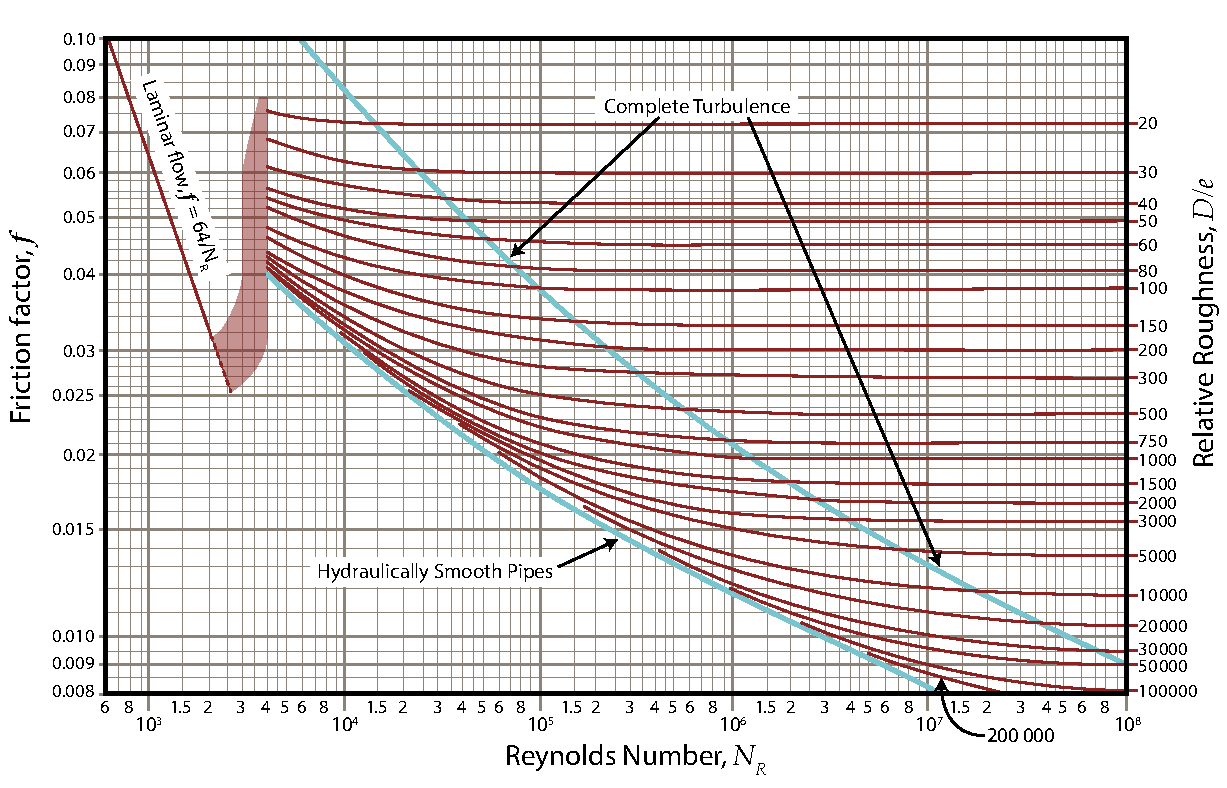
\includegraphics[scale=1.1, angle=90]{../../Figs/05FrictionLosses/moody.pdf}
\end{center}

\newpage


\begin{multicols}{2}
\par\bigskip
\textbf{Exit Loss} (i.e. exiting a pipe into a tank where all velocity is lost):
$$ K = 1 \Rightarrow h_L = \frac{v^2}{2g} $$

\par\vspace{1cm}
\hrule\par\bigskip

\textbf{Friction Factor, $\bm {f_T}$} in the zone of complete turbulence for new clean commercial \textbf{steel} pipe:
\par\bigskip
\begin{center}
	\begin{tabular}{>{$}r<{$} >{$}r<{$} >{$}l<{$} >{$}c<{$} >{$}r<{$} >{$}r<{$} >{$}l<{$}}
		\toprule
		\text{Nominal} & \quad & f_T &\qquad\qquad\qquad& \text{Nominal} & \quad & f_T\\
		\text{Size (in)} &&&& \text{Size (in)} &&\\
		\midrule
		\midrule
		\frac{1}{2} &&	0.027 && 3\frac{1}{2},4 &&	0.017\\
		\addlinespace	\midrule \addlinespace
		\frac{3}{4} &&	0.025 && 5 &&	0.016\\
		\addlinespace	\midrule \addlinespace
		1 &&	0.023 && 6 &&	0.015\\
		\addlinespace	\midrule \addlinespace
		1\frac{1}{4} &&	0.022 && 8-10 &&	0.014\\
		\addlinespace	\midrule \addlinespace
		1\frac{1}{2} &&	0.021 && 12-16 &&	0.013\\
		\addlinespace	\midrule \addlinespace
		2 &&	0.019 && 18-24 &&	0.012\\
		\addlinespace	\midrule \addlinespace
		2\frac{1}{2},3 &&	0.018\\
		\bottomrule
	\end{tabular}
\end{center}

\par\vspace{1cm}
\vfill\columnbreak
\begin{center}
\textbf{Equivalent-length ratios for valves}:

	\begin{tabular}{r >{$}r<{$} >{$}l<{$} >{$}c<{$} }
		\toprule
		\text{Type} & \quad & L_e/D \\
		\midrule
		Globe valve --- fully open &&	340 \\
		\addlinespace
		Angle valve --- fully open && 150\\
		\addlinespace
		Gate valve --- fully open &&	8 \\
		\addlinespace
		--- $3/4$ open && 35\\
		\addlinespace
		--- $1/2$ open && 160\\
		\addlinespace
		--- $1/4$ open && 900\\
		\addlinespace
		Check valve --- swing type  && 100\\
		\addlinespace
		Check valve --- ball type  && 150\\
		\addlinespace
		Butterfly valve --- fully open  && 45\\
		\addlinespace
		Foot valve --- poppet disc type  && 420\\
		\addlinespace
		Foot valve --- hinged disc type  && 75\\
		\addlinespace

		\bottomrule
	\end{tabular}
\end{center}

\par\vspace{1cm}
\textbf{Table of Equivalent-Length Ratios for Fittings}

\begin{tabular}{r >{$}r<{$} >{$}l<{$} >{$}c<{$} }
		\toprule
		\text{Type} & \quad & L_e/D \\
		\midrule
		$90\degree$ standard elbow &&	30 \\
		\addlinespace
		$90\degree$ long radius elbow &&	20 \\
		\addlinespace
		$90\degree$ street elbow &&	50 \\
		\addlinespace
		$45\degree$ standard elbow &&	16 \\
		\addlinespace
		$45\degree$ street elbow &&	26 \\
		\addlinespace
		Close return bend &&	50 \\
		\addlinespace
		Standard tee --- flow through run &&	20 \\
		\addlinespace
		Standard tee --- flow through branch &&	60 \\
		\addlinespace
		\bottomrule
	\end{tabular}
%%%%%%%%%%%%%%%%%%%%%%%%%%%%%%%%%%%%%%%%%%%%%%%%%%%%%%%%%%%%%%%%%%%%%%%%%%%%%%%%%%%%%%%%%%%%%%%%%%%%%%%%%%%%%%%%%%%%%

%\rule{\textwidth}{0.02in}
%%%%%%%%%%%%%%%%%%%%%%%%%%%%%%%%%%%%%%%%%%%%%%%%%%%%%%%%%%%%%%%%%%%%%%%%%%%%%%%%%%%%%%%%%%%%%%%%%%%%%%%%%%%%%%%%%%%%%
% \end{multicols}{2}
\newpage
% \begin{multicols}{2}
\raggedright

%%%%%%%%%%%%%%%%%%%%%%%%%%%%%%%%%%%%%%%%%%%%%%%%%%%%%%%%%%%%%%%%%%%%%%%%%%%%%%%%%%%%%%%%%%%%%%%%%%%%%%%%%


	\textbf{Example 1}:
	\par\medskip

	Determine the head loss that occurs when $100\text{ L/min}$ of fluid flows from $3\text{-in}$ Type K copper tube $(D=73.84\,\text{mm})$ into
	$1\text{-in}$ Type K copper tube $(D=25.27\,\text{mm})$ through a sudden contraction.

	\textbf{Solution}:\\

	\cbox[0.9]{
		From the sudden contraction K-value table, $\mathsf{D_1}$ is the larger pipe diameter and $\mathsf{D_2}$ the smaller
		pipe diameter so

		\[ \frac{D_1}{D_2} = \frac{73.83\,\text{mm}}{25.27\,\text{mm}} \approx 2.9 \]

		The velocity in the smaller pipe is
		\begin{align*}
			v_2 &= \frac{Q}{A} \\
			&= \frac{0.1/60\,\mathsf{m^3/s}}{\pi(0.02527\,\text{m})^2/4} \\
			&= 3.3231\,\text{m/s}
		\end{align*}

		From the table:
		\[ k \approx 0.42 \]

		Then,

		\begin{align*}
			h_L &= k\cdot\frac{v^2}{2g} \\
			&= 0.42 \cdot \frac{(3.3231\,\text{m/s})^2}{19.62\,\mathsf{m/s^2}}\\
			&= 0.23639\,\text{m}\\
			&\approx 0.236\,\text{m}
		\end{align*}
	}

 	\vfill

\columnbreak
%%%%%%%%%%%%%%%%%%%%%%%%%%%%%%%%%%%%%%%%%%%%%%%%%%%%%%%%%%%%%%%%%%%%%%%%%%%%%%%%%%%%%%%%%%%%%%%%%%%%%%%%%%%%%%%%%%%%%



\textbf{Example 2}:

Determine the head loss for a gradual contraction from $4\text{-in}$~Schedule~$80$~pipe $(D=97.2\,\text{mm})$ to a
$1\tfrac{1}{2}\text{-in}$ Schedule $80$ pipe $(D=38.1\,\text{mm})$ with a cone angle of $76\degree$.
\lb The flow is $450\text{ L/min}$.

\textbf{Solution}:

\cbox[0.9]{
	For $\theta=76^\circ$,
	\begin{align*}
		k &= 0.5\sqrt{\sin\frac{\theta}{2}}\left(1-\left(\frac{D_2}{D_1}\right)^2\right) \\
		&= 0.5\sqrt{\sin \frac{76^\circ}{2}}\left(1-\left(\frac{38.1\,\text{mm}}{97.2\,\text{mm}}\right)^2\right)\\
		&= 0.33204
	\end{align*}

	Velocity and velocity head in the smaller downstream pipe:

	\begin{align*}
		Q &= \frac{450/60\,\mathsf(m^3/s)}{\pi(0.0381\,\text{m})^2/4}\\
		&= 6.5784\,\text{m/s}\\\\
		\frac{v^2}{2g} &= 2.2057\,\text{m}
	\end{align*}

	Then,

	\begin{align*}
		h_L &= k\cdot\frac{v^2}{2g} \\
		&= 0.33204 \times 2.2057\,\text{m}\\
		&\approx 0.732\,\text{m}
	\end{align*}

}

\vfill
\pagebreak

%%%%%%%%%%%%%%%%%%%%%%%%%%%%%%%%%%%%%%%%%%%%%%%%%%%%%%%%%%%%%%%%%%%%%%%%%%%%%%%%%%%%%%%%%%%%%%%%%%%%%%%%%%%%%%%%%%%%%
\textbf{Example 3}:

Determine the head loss that occurs when $100\text{ L/min}$ flows from $1\text{-in}$ Type K copper tube $(D=25.27\,\text{mm})$ into
$3\text{-in}$ Type K copper tube $(D=73.48\,\text{mm})$ through a sudden enlargement.

\textbf{Solution}:

\cbox[0.9]{

Again, losses are based on the velocity head in the smaller (in this case, upstream) pipe.

\begin{align*}
	v_1 &= \frac{0.1/60\,\mathsf{m^3/s}}{\pi(0.02527\,\text{m})^2)/4} \\
	&= 3.3231\,\text{m/s}\\\\
	\frac{v^2}{2g} &= 0.56286\,\text{m}\\\\
	\frac{D_2}{D_1} &= \frac{73.84\,\text{mm}}{25.27\,\text{mm}} \\
	&= 2.9220
\end{align*}

Velocity is greater than 1.2 m/s so we use the table to find that $K \approx 0.73 $

\begin{align*}
	h_L &= K\cdot\frac{v^2}{2g} \\
	&= 0.73\times 0.56286\,\text{m} \\
	&\approx 0.411\,\text{m}
\end{align*}

}

\vfill
\columnbreak
%%%%%%%%%%%%%%%%%%%%%%%%%%%%%%%%%%%%%%%%%%%%%%%%%%%%%%%%%%%%%%%%%%%%%%%%%%%%%%%%%%%%%%%%%%%%%%%%%%%%%%%%%%%%%%%%%%%%%

\textbf{Example 4}:

Compare the headlosses between an inward-projecting entrance and rounded entrance with a radius of $25\text{ mm}$
for water entering $6\text{-in}$ Schedule 40 steel pipe $(D=154.1\,\text{mm})$ with a flow of $75\text{L/s}$. (Use $K=0.78$.)

\textbf{Solution}:

\cbox[0.9]{

	\begin{align*}
		v &= \frac{0.075\,\mathsf{m^3/s}}{\pi(0.1541\,\text{m})^2)/4} \\
		&= 4.0213\,\text{m/s}\\\\
		\frac{v^2}{2g} &= 0.82420\,\text{m}	\\\\
		\intertext{For inward projecting entrance:}
		h_L &= 0.78\times 0.82420\,\text{m} \\
		&= 0.64288\,\text{m}\\\\
		\intertext{For rounded entrance:}
		\frac{r}{D} &= \frac{25\,\text{mm}}{154.1\,\text{mm}}\\
		&= 0.16223 \\
		\Rightarrow K &= 0.04\\\\
		\intertext{Then head loss is given by:}
		h_L &= K\cdot\frac{v^2}{2g}\\
		&= 0.032968\,\text{m}
	\end{align*}

}


\vfill
\pagebreak

%%%%%%%%%%%%%%%%%%%%%%%%%%%%%%%%%%%%%%%%%%%%%%%%%%%%%%%%%%%%%%%%%%%%%%%%%%%%%%%%%%%%%%%%%%%%%%%%%%%%%%%%%%%%%%%%%%%%%
	\textbf{Example 5}:

	Find the pressure drop across a fully open globe valve ($L_e/D=340$) in $4\text{-in}$ Shedule $40$ steel pipe $(D=102.3\,\text{mm})$
	carrying $1600\text{ L/min}$.

	\textbf{Solution}:

	\cbox[0.9]{

	We have a number of options to find $f_T$: the Moody diagram, the Swamee-Jain formula and directly
	from the table for values of $f_T$ for new commercial steel. (The table gives a value of $f_T=0.017$.)

	The relative roughness is:
	\[ \frac{D}{\epsilon} = \frac{0.1023\,\text{m}}{4.6\times 10^{-5}\,\text{m}} = 2223.9 \]

	Using the Moody diagram, we choose a value for the Reynold's number anywhere in the zone of complete turbulence for a
	relative roughness of $2223.9$. Reading the friction factor from the left hand side of the diagram gives $f_T\approx
	0.0165$

	Using the Swamee-Jain Formula with $N_R = 3.6\times10^6$, where flow with a relative roughness of $2223.9$ becomes
	completely turbulent:

	\begin{align*}
		f_T &= \frac{0.25}{\left[\log\left(\frac{1}{3.7\left(D/\epsilon\right)}+\frac{5.74}{N_R^{0.9}}\right)\right]^2}  \\\\
		&=
		\frac{0.25}{\left[\log\left(\frac{1}{3.7\left(2223.9\right)}+\frac{5.74}{\left(3.6\times10^6\right)^{0.9}}\right)\right]^2}
		\\\\
		&= 0.016519
	\end{align*}

	The three results for $f_T$ are within 3\% of each other, which is more accurate than we expect from any calculations
	of flow so these are effectively the same result.

	For new commercial steel pipe, using the appropriate table is convenient. Beware, though, that you don't use it for any
	other type of pipe or tubing.

	}

	\vfill\columnbreak

	\cbox[0.9]{

		Now, we can find the resistance coefficient, $K$, of the valve for this pipe:

	\[ K = f_T\cdot\frac{L_e}{D} = 0.017\times 340 = 5.78 \]

	The velocity and velocity head are:

	\begin{align*}
		v &= \frac{1.6/60\,\mathsf{m^3/s}}{\pi(0.1023\,\text{m})^2/4}\\
		&= 3.2443\,\text{m/s}\\\\
		\frac{v^2}{2g} &= 0.53648\,\text{m}
	\end{align*}

	Head loss across the valve is given by:

	\begin{align*}
		h_L &= K\cdot\frac{v^2}{2g}\\\\
		&= 5.78\times 0.53648 \\\\
		&= 3.1008\,\text{m}
	\end{align*}

	Use the GEE to find the pressure drop:

	\begin{align*}
		\frac{P_1}{\gamma} - h_L &= \frac{P_1}{\gamma} \\\\
		P_1-P_2 &= \gamma\cdot h_L \\\\
		&= 9.81\,\mathsf{kN/m^3}\times 3.1008\\\\
		&= 30.4\,\text{kPa}
	\end{align*}

	}

	\vfill\pagebreak

%%%%%%%%%%%%%%%%%%%%%%%%%%%%%%%%%%%%%%%%%%%%%%%%%%%%%%%%%%%%%%%%%%%%%%%%%%%%%%%%%%%%%%%%%%%%%%%%%%%%%%%%%%%%%%%%%%%%%
	\textbf{Example 6}:

	Calculate the headloss across a ball-type check valve placed in a $1\tfrac{1}{4}\text{-in}$ copper
	tubing $(D=31.62\,\text{mm})$ if water is flowing through the tubing with a velocity of $2.35\text{ m/s}$.

	\textbf{Solution}:

	\cbox[0.9]{

		The relative roughness is:

		\[ \frac{D}{\epsilon} = \frac{0.03162\,\text{m}}{1.5\times 10^{-6}\,\text{m}} = 21087 \]

		Copper tubing so we need either the Moody diagram or the Swami-Jain. From the Moody diagram:
		\[ f_T = 0.0105 \]

		The resistance coefficient, $K$, of the valve for this pipe:

		\[ K = f_T\cdot\frac{L_e}{D} = 0.0105\times 150 = 1.575 \]

		The velocity head is:

		\[ \frac{v^2}{2g} = \frac{(2.35\,\text{m/s})^2}{19.62\,\mathsf{m/s^2}} = 0.28147\,\text{m} \]

		Head loss across the valve is given by:

		\begin{align*}
			h_L &= K\cdot\frac{v^2}{2g}\\\\
			&= 1.575\times 0.28147 \\\\
			&= 0.44332\,\text{m}
		\end{align*}

	}


	\vfill\columnbreak

%%%%%%%%%%%%%%%%%%%%%%%%%%%%%%%%%%%%%%%%%%%%%%%%%%%%%%%%%%%%%%%%%%%%%%%%%%%%%%%%%%%%%%%%%%%%%%%%%%%%%%%%%%%%%%%%%%%%%
	\textbf{Example 7}:

	Find the pressure drop across a $90\degree$ standard elbow in a $2\tfrac{1}{2}\text{-in}$ Schedule $40$ steel pipe $(D=62.7\,\text{mm})$ if water is flowing
	at the rate of $800\text{ L/min}$.

	\textbf{Solution}:

	\cbox[0.9]{

		From the table of $f_T$ values for new commercial steel pipe, $f_T=0.018$

		Then

		\begin{align*}
			v &= \frac{0.8/60\,\mathsf{m^3/s}}{\pi(0.0627\,\text{m})^2/4}\\
			&= 4.3183\,\text{m/s}\\\\
			\frac{v^2}{2g} &= 0.95045\,\text{m}\\\\
			K &= f_T\cdot\frac{L_e}{D}\\
			&= 0.018\times 30\\
			&= 0.54\\\\
			h_L &=  K\cdot\frac{v^2}{2g}\\
			&= 0.54\times 0.95045 \\
			&= 0.51324\,\text{m}\\\\
			P_1-P_2 &= \gamma\cdot h_L \\
			&= 9.81\,\mathsf{kN/m^3}\times 0.51324\\
			&= 5.0349\,\text{kPa}
		\end{align*}
	}


	\vfill\pagebreak


\end{multicols}
\end{document}
